\subsection{Segmentação}

O estudo de segmentação dentro da área de redes neurais convolucionais começou a partir de redes totalmente convolucionais que descarta a camada totalmente conectada visto que a saída deverá ser uma imagem e não uma classificação. Uma arquitetura muito utilizada em modelos de segmentação é a Encoder-Decoder, que separa em dois passos: o primeiro para convergir no mapa de características e o segundo para reverter em uma imagem usando camadas desconvolucionais e desagrupamento. Existem três principais nichos sendo eles: segmentação semântica que é a classifiicação por pixels, a segmentação de instância que atribui um id para cada objeto encontrado de uma classe e a segmentação panóptica que junta as duas anteriores para criar uma imagem semelhante a saída de segmentação semântica porém separando objetos de mesma classe sendo essa a mais recente, exemplificando com \cref{fig:segentacoes} \cite{dp_semantic_segmantation, lapix}. 

\begin{figure}[H]
	\caption{Tipos de segmentação em redes neurais convolucionais}
	\centering % para centralizarmos a figura
	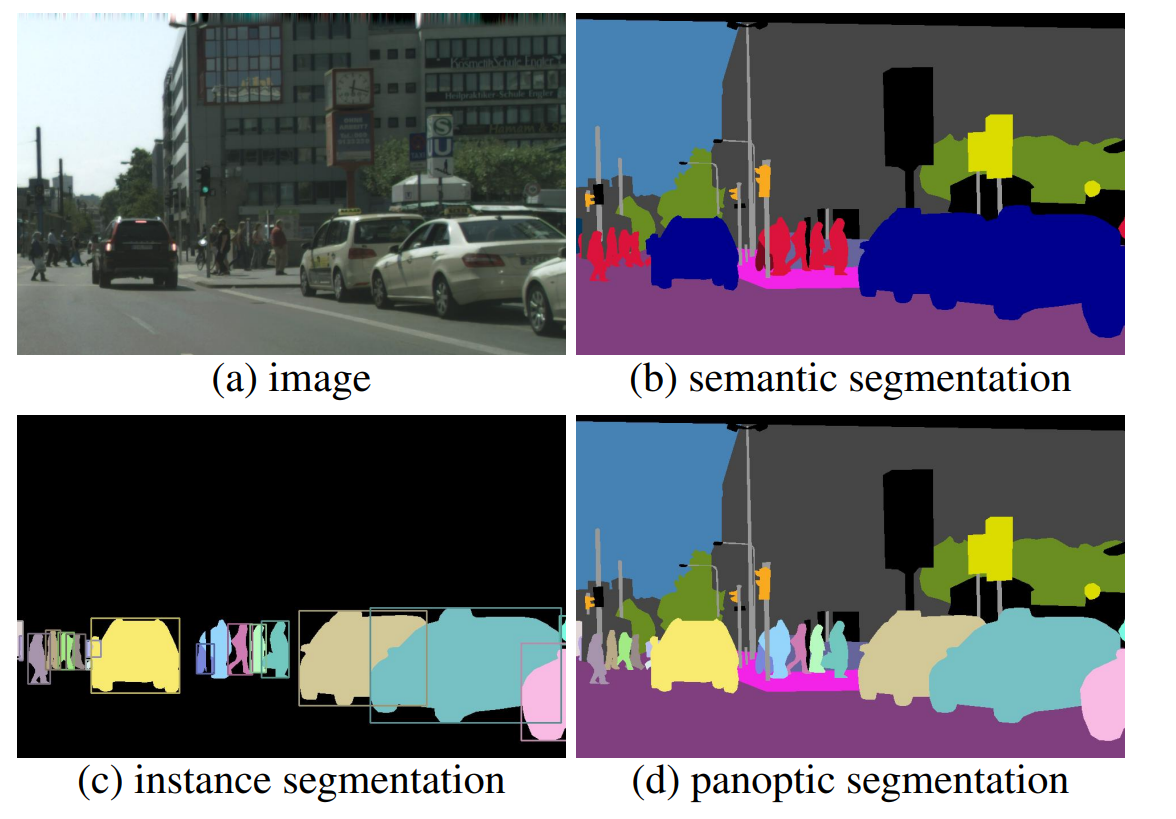
\includegraphics[width=10cm]{figures/segmantations.png} % leia abaixo
	\legend{Fonte: \citeonline{kirillov2019panoptic}}
	\label{fig:segentacoes}
\end{figure}

Com base na imagem acima percebemos que segmentação panóptica é a melhor opção para nossa aplicação além do fato de ser a mais nova. Portanto abordaremos métricas para escolher um modelo dentro dessa área de estudo.



Variações de arquiteturas